\documentclass[%	draftcls,	% Remove when document becomes final!
				12pt,
				a4paper,
				twoside,
				titlepage,
				headsepline,
				numbers=noenddot,
				listof=totoc,
				index=totoc,
				bibliography=totoc]{scrartcl}


\ifx\pdfoutput\undefined
\pdffalse % we are not running pdflatex
\else
\pdfoutput=1 % we are running pdflatex
\pdfcompresslevel=9     % compression level for text and image;
\usepackage[juratotoc]{scrjura}
\usepackage[pdftex,
	bookmarks=true,
	bookmarksopen=false,
	bookmarksnumbered=true,
	linktocpage,colorlinks=true,
	backref,
	pagebackref,
	linkcolor=black,
	citecolor=black,
	urlcolor=black]{hyperref}
\usepackage[pdftex]{graphicx}
\usepackage{microtype}
\fi

\usepackage{amsfonts}
\usepackage{algorithmic}
\usepackage[english]{babel}
\usepackage{url}
\usepackage{color}
\usepackage{tabularx}
\usepackage[T1]{fontenc}
\usepackage[latin1]{inputenc}
\usepackage{bbm}
\usepackage{amsmath}
\usepackage{amssymb}
\usepackage{ntheorem}
\usepackage{microtype}
\usepackage[htt]{hyphenat}
\usepackage{fancyvrb}
\usepackage{subfigure}
\usepackage{mathptmx} 
\usepackage[scaled=.90]{helvet} 
\usepackage{courier}
\usepackage[rightcaption]{sidecap}
\usepackage{lscape}
\usepackage{supertabular}
\usepackage{everysel}

\usepackage[footnote]{acronym}

\usepackage[obeyDraft]{todonotes}
\usepackage{xifthen}
\usepackage{fancyhdr}

\usepackage{color, colortbl}
\usepackage{xcolor}
\usepackage{pifont}

\usepackage{longtable}
\usepackage{enumitem}

\usepackage{rotating}

\usepackage{morefloats}

\usepackage{listings}

\usepackage{parskip}

\RequirePackage{xspace}

\setcounter{secnumdepth}{3}

\newcommand{\p}[1]{\texttt{\small #1}}

\theoremstyle{break}
\newtheorem{ex}{Example}[section] 

\definecolor{gray}{gray}{0.95}
\definecolor{darkgreen}{RGB}{0,127,0}
\definecolor{darkyellow}{RGB}{255,210,0}
\setlength{\fboxrule}{2pt}

\providecommand{\ext}[1]{}

\pagestyle{fancy}
\renewcommand{\sectionmark}[1]{\markright{\thesection\ #1}}
\fancyhf{}
\rhead{\fancyplain{}{}}
\lhead{\fancyplain{}{\rightmark }} 
\cfoot{\fancyplain{}{\thepage}}

\newacro{evolutionary case study}[evolutionary case study]{\emph{Case Study which keeps on evolving with time}}
\newacro{demo}[demo]{\emph{short for Demonstration}}
\newacro{UML}[UML]{\emph{short for Unified Modeling Language}}
\newacro{UI}[UI]{\emph{short for User Interface}}
\newacro{Eclipse}[Eclipse]{\emph{Integrated Development Environment (IDE) for programming Java}}

\begin{document}                

	\begin{titlepage}
	\thispagestyle{empty}
	\begin{center}

			
\includegraphics[width=12cm]{figures/Logo_Uni_Paderborn}\\
                      
      		\vspace{3cm}
			{\LARGE  \text{Master's Thesis Proposal}} \\
			\vspace{0,3cm}
			\text{on} \\
			\vspace{0,3cm}
			{\LARGE  \textbf{A Demonstrator Framework\\ 
					for Consistency Management Approaches}} \\ 
			\vspace{1cm}
			\text{by} \\
			\vspace{0,3cm}
			\begin{tabular}{l l}
				Student: & Arjya Shankar Mishra \\
				Matriculation No.: & 6772832\\
			\end{tabular}\\	
			\vspace{3cm}
			\begin{tabular}{l l}
				Supervisor: & Jun. Prof. Dr. Anthony Anjorin \\ \\ \\
			\end{tabular}\\ 
			\vspace{3cm}	
			\begin{tabular}{l l}
				Paderborn, \today \\
			\end{tabular}\\	
					
	\end{center}
	\end{titlepage}
	\clearpage

  
  	\pagenumbering{arabic}
	\setcounter{page}{2}
	
	% ************************************************************
	% *****                    Content                        *****
	% ************************************************************
  
  	\section{Introduction}\label{sec:introduction}
In recent times \textit{bidirectional transformation} (denoted by "bx") has gained importance in the field of Model-Driven Software Development \cite{bx-grace} \cite{bx-dagstuhl}. BX is a technique used to synchronize two (or more) instance of different meta-models. Both models are related, but don't necessarily contain the same information. Changes in one model thus lead to changes in the other model \cite{bx-grace}. 
\newline\newline\textit{Bidirectional transformation} is used to deal with scenarios like:
\begin{itemize}
	\item {change propogation to user interface as a result of underlying data changes}	
	\item {synchronization of business/software models}
	\item {refreshable data-cache incase of database changes}
\end{itemize}
    and many more....
\newline\newline Bx community has been doing research and development work in many fields like software development, database, mathematics and many more to increase awareness and to reach more people \cite{bx-dagstuhl}\cite{bx-grace}. As a result, many kinds of bx tools are being developed, e.g., eMoflon \cite{emoflon-part4}, Echo \cite{echo}. These bx tools are based on various approaches, such as, graph transformations, bidirectionalization, update propagations \cite{bx-community} and can be used in different areas of application.
\newline\newline One basic problem that still persists is that the knowledge of and awareness for "bx" is limited. In this thesis, my goal is to design and implement an interactive demonstrator based on an example. An existing bx tool will be used as a part of the demonstrator to realize \textit{bidirectional transformation}. The final prototype will be interactive and easily accessible to users to help them understand the potential, power and limitations of bx.
\newline\newline This proposal is structured as follows: Section 2 describes the problem that I will address in my thesis. Section 3 presents the current state of the art and existing pain points. Based on this, in Section 4, research questions will be explained that I will be trying to solve in my thesis. Section 5 describes the research method. Section 6 describes the examples that can be implemented and the architecture design. Section 7 presents the time plan. Finally, Section 8 presents a tentative structure of the final thesis.



  	\newpage
  	\section{Problem Description}\label{sec:problem}
\textit{Bidirectional transformation} is an emerging concept. In the past, many efforts have been made by conducting international workshops, seminars and through experiments conducted by developers / bx community to identify its potential. Also, in addition to the development of bx tools and bx language, benchmarks are being created for bx tools for systematic comparison \cite{benchmark-BX}.
\newline\newline  Although a significant amount of work has been done in this field, some basic problems still remain:
\begin{itemize}
	\item {Reachability to relevant communities is not significant due to the absence of a common vocabulary for bx across research disciplines \cite{bx-theoryandappl}. Seminars are still conducted for exchanging ideas in different communities to define a common vocabulary of terms and properties for bx \cite{bx-dagstuhl}.}	
	\item {Bx tools and their applicability is still not widely known even in the developers' communities. Due to the existing conceptual and practical challenges associated with using bx, bx-tools in building software systems, many developers and researchers are still using non-bx transformation tools to achieve properties which can be easily supported by bx-tools \cite{bx-theoryandappl}.}
	\item {Absence of a simple yet interactive bx tool demonstrator to depict the potential of \textit{bidirectional transformation} over preferred non-bx tool demonstrators among developers' and researchers' communities \cite{bx-theoryandappl}.}
\end{itemize}

\section{State of the Art}\label{sec:stateofart}
Model transformation is a central part of Model Driven Development. The main concept of synchronization is to propagate changes from some model to other related models.
\newline\newline Nowadays, researchers from different areas are actively investigating the use of bx to solve a variety of problems. A lot of work has been done in terms of building usable tools and languages for bx. These tools can be used in various fields, for achieving \textit{bidirectional transformation}. To understand these tools, several handbooks, tutorials and examples have been created so that users and developers can understand the core concepts. 
\subsection{Handbooks \& Tutorials}\label{subsec:handbook}
 As a part of our research, we have analyzed some tutorials and tools and below are our findings.
\newline\newline Anjorin et al.\cite{emoflon-part4} present the concept for \textit{bidirectional transformation} using Triple Graph Grammars (denoted by "TGG") \cite{tgg}. To demonstrate their core idea and the usage of the tool, they have described an example by transforming one model (source) into another (target) through TGG transformations \cite{tgg}\cite{bx-tgg}. The whole tutorial is about 42 pages long which guides the user to get the example running through a series of steps. These steps include, installing \ac{Eclipse}, getting their tool as a Eclipse plugin, setting up the workspace, creating TGG schema and specifying it's rule and much more. If the user is able to execute each step correctly, then finally he/she can view the final output. It took me 4 days to get the tool up and running.
\newline\newline We have analyzed a tutorial\cite{bigul-tutorial} on a bidirectional programming language BiGUL\cite{bigul}. The core idea with BiGUL is to write only one putback transformation, from which the unique corresponding forward transformation is derived for free. The whole tutorial is about 45 pages long which includes a lot of complex formulas, algorithms and guides the user to get the example running through a series of steps. These steps include, installing BiGUL, setting up the environment, achieving bx through BiGUL's bidirectional programming and much more. If the user is able to execute each step correctly, then finally he/she can view the final output. 
\newline\newline However, the whole process described in the above paragraphs to get the tool/example running are not that straight forward. Some associated problems that I found with the tutorials and handbooks are as follows: 
\begin{itemize}
	\item {Installation requires technical expertise and time consuming as the user typically has to setup and install the tool.}

	\item {Required knowledge is too tool/area specific, e.g., User must possess knowledge about Java and Eclipse framework or configuring the tool is not compatible with all the versions of Eclipse.}
	
	\item {Can be challenging if the user is not familiar with the technological space, e.g., a Java programmer might find the tool chain for Haskell unfamiliar, and vice-versa.}	
	
	\item {Steps for get the example running needed technical expertise, e.g., In some cases domain specific knowledge includes mathematics and specific coding language. What is showcased and discussed is tied to a specific technological space and might not be easily transferable to other bx approaches.}
	
	\item {Not very helpful to understand what bx is before deciding which bx tool (and corresponding technological space) to use.}
\end{itemize}
\subsection{Example Repositories}\label{subsec:examplerep}
A rich set of bx examples repository \cite{bx-examples} has been created based on many research papers. These examples cover a diverse set of areas such as business process management, software modelling, data structures, database, mathematics and many more.
\newline\newline User can find relevant information about the examples on the respective web pages. Some of the examples are very well documented along with class diagrams, activity diagrams, object diagrams etc. and source code of a few examples are available as well. 
\newline\newline In today's fast paced and visually enriched world, "what you see is what you believe" and that is exactly what these examples are lacking in. None of the examples have an online \ac{demo} showing how it works. Hence, it is very difficult for a user to realise the examples just by going through the documentation and \ac{UML} diagrams. Even if source code is present, it takes a lot of time and requires technical expertise to set-up the framework and get the example running.
\subsection{Existing Demonstrators}\label{subsec:existingdemo}
Also, we have analyzed an existing demonstrator available along with the test cases of domain-specific language, BiYacc \cite{biyacc} which is based on BiGUL \cite{bigul}. 
\newline\newline Being an online demonstrator, user can try it out instantly and check how it works. It doesn't require any installation or technical expertise to get the example running and also, it makes the features of bx noticeable.
\newline\newline But, the problems that we found out with the demonstrator are as follows: 
\begin{itemize}
	\item {The demonstrator's visual representation doesn't create interest in the target audience as it does not exploit the potential of using an interactive GUI and colors, etc. It just makes use of two text fields and is comparable to a console-based interface that is accessible online.}
	\item {The demonstrator is not intuitive for a large group of users as there is very limited guidance provided concerning what the user can do and try out with the demonstrator. Especially for non-experts, it is not clear what to do with the demonstrator after a few minutes.}
	\item {The demonstrator is based on a rather technical example that might not be relevant, interesting, or convincing for a large group of potential bx users.}		
\end{itemize}
\subsection{Virtual Machines}\label{subsec:virtualmachines}
Also, we have analyzed a web based virtual machine, e.g., SHARE \cite{share}. Basically, this is a web portal used for creating and sharing executable research papers and acts as a demonstrator to provide access to tools, softwares, operating systems, etc., which are otherwise a headache to install \cite{share}. 
\newline\newline This provides the environment that the user requires to execute his/her tool or program. Hence, it reduces the overhead of a user for maintaining and organising all software framework related stuff and simplify access for end-users.
\newline\newline But, the problem that we found with the virtual machine are as follows:
\begin{itemize}
	\item {For security reasons, it's not like other web portals where user need to simply sign-up and can host/create/access data, rather it includes a series of request-grant cycle for getting access to an environment and hosting/managing data. Also, some actions require special authorization and take time to complete the whole process.}
	\item {User needs at least 3 Gigabyte or more space on his/her local system for configuring the virtual machines depending on the requirement of the environment, which sometimes creates an overhead.}
\end{itemize}	
\section{Objectives}\label{sec:objectives}
The goal of this thesis is to explore the fundamental and technical challenges involved in implementing a demonstrator for bx tools.
\newline\newline This thesis aims at answering these main research questions:
\\\textbf{\textit{RQ1}} -- What are the core requirements for implementing a successful bx demonstrator ?\\
\\\textbf{\textit{RQ2}} -- What kind of interactivity and to what extend is it required in the bx demonstrator ?\\
\\\textbf{\textit{RQ3}} -- Which goals can be particularly well addressed in a bx demonstrator and why ?\\
\\\textbf{\textit{RQ4}} -- To what extent is such a bx demonstrator reusable?\\
RQ4 can be split into the following sub-questions:
\\\textbf{\textit{RQ4.1}} -- Is the implementation of the demonstrator bx tool-specific ?\\
\\\textbf{\textit{RQ4.2}} -- Is the implementation of the demonstrator example-specific?\\
\\\textbf{\textit{RQ4.3}} -- What part(s) of the demonstrator can be reused in implementing a different example ?
\newline\newline All of my work will be directly or indirectly related to the above research questions.

\section{Research Method}\label{sec:research}
Our work is based on an \ac{evolutionary case study} which focuses on designing and implementing a successful bx tool demonstrator. Our entire work cycle is described in the following paragraphs.
\paragraph{Case Study}
Initially, the case study will be based on the existing bx tools on the market, flexibility in usage, time and technical expertise required to use these bx tools, and the implementation of these tools in different areas. With the initial study and knowledge gathered, we will evaluate the requirements as described in Section \ref{sec:objectives} for improving the existing situation and the usefulness of the demonstrator.
\paragraph{Examples and Implementation}
To realize the requirements, we will construct a few examples which can be implemented covering the requirements and showing the usability of bx tools through demonstrator. Then we will choose the best suitable example to implement and build the final prototype.
\paragraph{Evaluation} To evaluate the demonstrator, we will conduct a feedback session with groups of users. According to the availability and reachability, the users can be experts on bx, students of a Model-Driven Software Development/Engineering course, friends and colleagues with computer science background. We will let the users to try the prototype and get feedback either through online questionnaires or through personal interviews.
\newline\newline Based on the feedbacks from the users, we will update our learning goals and check how far we have succeeded in fulfilling the requirements. If results are not satisfactory, then another iteration will be done i.e. further refinement to the case studies, example to implement and implementation.
\paragraph{Choices and Threats} 
The implementation process and the final prototype will be driven by many choices and threats. For example, the selection of the bx tool and the most suitable example to implement will decide the usefullness of the demonstrator. My decisions on designing the framework for implementation, seleting the bx tool and example to implement will be influenced by the ideas given by my supervisor. During evaluation, I might not get proper feedback from my friends \& colleagues due to my acquaintance.
\newline\newline Number of iterations conducted for getting satisfactory result will depend on the complexity of the implementation and availability of time after first successful implemenation.

\section{Idea and Implementation}\label{sec:implementation}
Due to the existing pain points with the bx tools as described in Section \ref{sec:stateofart} and to solve the problems as described in Section \ref{sec:problem}, the main idea is to design and implement an interactive bx tool demonstrator.
\subsection{Choosing an Example}\label{subsec:examples}
As of now we have discussed a few examples as follows:
\paragraph{Task Management} This prototype can be used for allocating tasks in a team. It contains two views e.g., supervisor's view and employee's view. A Supervisor can allocate tasks to their sub-ordinates. An employee can view the tasks assigned to him. Then the task will go through a life cycle as the work progresses, i.e., Assigned, In Progress, Testing, Done. Supervisor's view shows aggregate information from multiple projects and multiple employees, but does not contain detailed information, e.g., tasks have fewer states than for assigned employees. Bx rules control how updates are handled and states are reflected in the different views of the project, e.g., the employee's view will be updated for each state change, whereas the supervisor's view is only updated when a task is completed and not for intermediate changes.

\paragraph{Quiz} This prototype can be used for an online quiz game. It contains two views e.g., administrator's view and participant's view.
There will be a large set of questions related to different areas, e.g, history, geography, politics, sports, etc. The administrator can select the areas from which the questions will be shown to the participant and initiate the game. The participant can override the selection of the areas and start the quiz. Randomly questions will be shown to the participant from the selected areas with 4 options. The administrator's view contains less information than the participant's view, e.g., only the result of each question will be shown to the administrator, whereas participant can see questions along with its options. As soon as the participant chooses the answer to any question, bx rules control how updates are handled and states are reflected in the different views of the project.

\paragraph{Playing with Shapes} It contains two views e.g., low level view (depicts \ac{UI} for low level language, i.e., UI with less functionality) and high level view (depicts UI for high level language, i.e., UI with more functionality). User will draw a geometric shape, i.e., triangle / square / rectangle / circle with some notations similar to the shape on the low level view and if the notations are correct, the high level view tries to recognize the shape and draws it with default parameters and vice-versa. Basically the transformation will happen between a low level language and a high level language and bx rules control how updates are handled and states are reflected in the different views of the project. In high level view, more functionalities will be present, i.e., moving one shape from one place to another, creating a clone of an existing shape, etc. which is not possible in low level view.

\subsection{Architectural Representation}\label{subsec:archirep}
High-level architecture of my prototype in form of a component diagram  is given in Figure~\ref{fig:Component_Diagram}.
\begin{figure}
	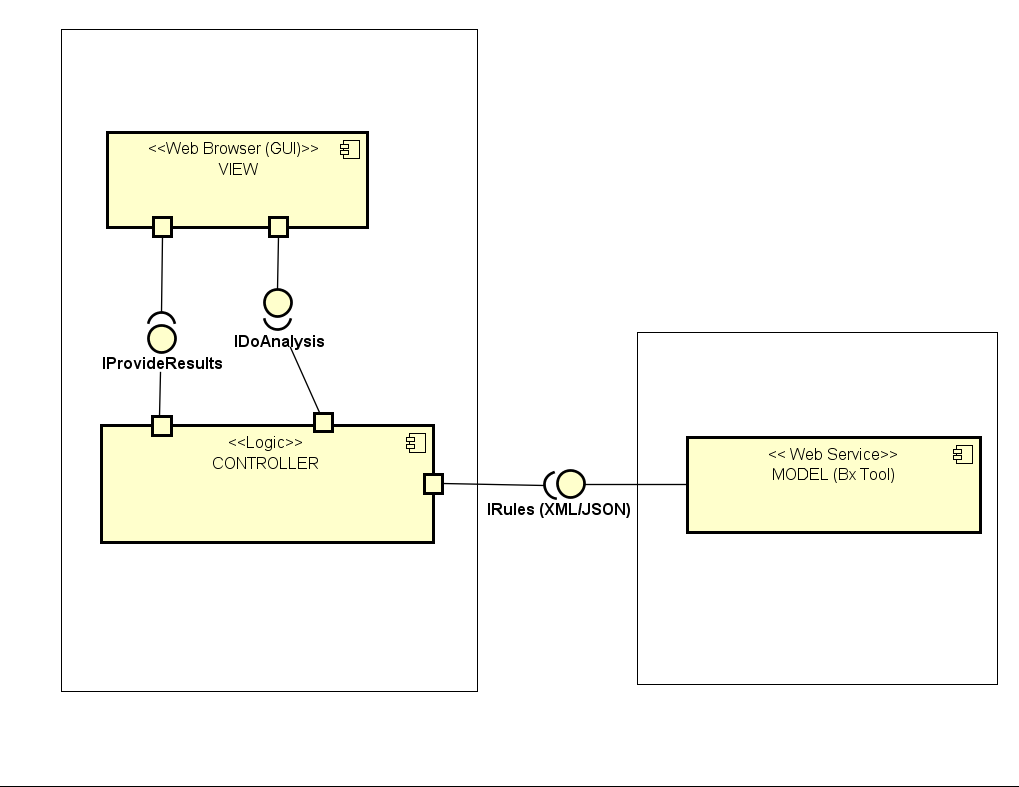
\includegraphics[width=1\textwidth]{figures/Component_Diagram}
	\caption{Component Diagram}
	\label{fig:Component_Diagram}
\end{figure}

I am using Model-View-Controller (MVC) pattern for my application framework. 
On the top, \texttt{View} (Web Browser) component is present which contains a graphical user interface and functionalities that belong to the user. With the changes on \texttt{View} component, data are being provided through interface \texttt{IDoAnalysis} to the \texttt{Controller} component and after the calculations are done, the results are sent back to the \texttt{View} through interface \texttt{IProvideResults}. Both \texttt{View} and \texttt{Controller} resides on the same machine.
\newline\newline \texttt{Model} (Bx Tool) component resides on a separate machine and communicate via web services. It encapsulates and manages the state of all models by communication with the \texttt{Controller} through interface \texttt{IRules} in the form of XML or JSON format.
  	\newpage
  	\section{Plan and Schedule}\label{sec:timeplan}
The time schedule, mentioned below, is only provisional and might change
during development process by {$\pm$}10\% of the total time.

\begin{center}
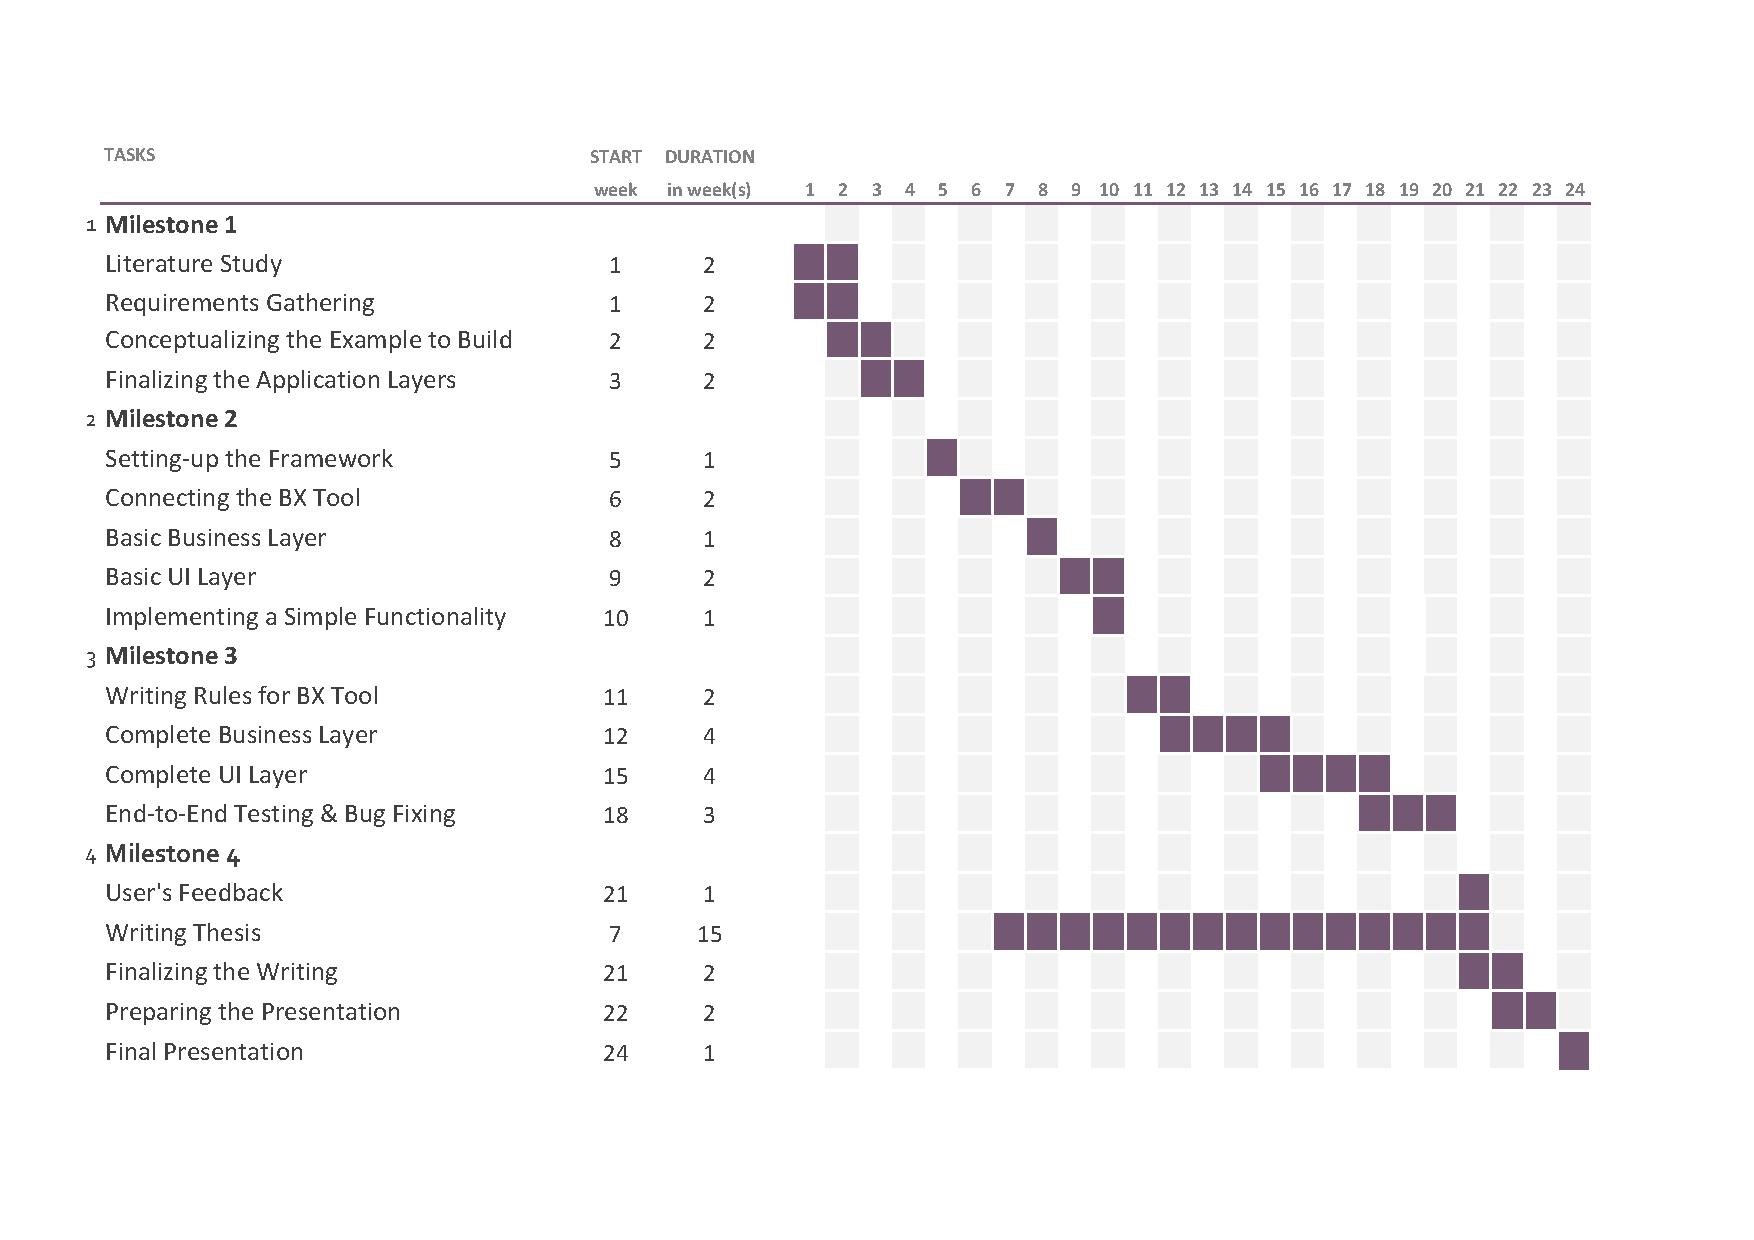
\includegraphics[width=1.1\textwidth]{figures/Time_Plan}
\captionof{figure}{Time Plan}
\label{fig:time_plan}
\end{center}

\section{Preliminary Structure of Final Documentation}\label{sec:finaldocument}
Below is the tentative structure of the document that will be available after the completion of the thesis.
\begin{enumerate}
	\item {Introduction}
	\item {Motivation}
	\item {Background and Related Work}
	\item {Research Method}
	\item {Architecture Design}
	\begin{itemize}
	    \item {High level architecture information}	
	    \item {Concrete design decision}
	    \item {UML Diagrams}
	\end{itemize}
	\item {API}
	\item {Application Walkthrough}
	\item {Outcome of Research Method: Feedback, Discussion and Learning Goals}
	\item {Future Work}
	\item {Conclusion}
\end{enumerate} 
* \textit{Above is just a preliminary and tentative structure and may vary.}

\begin{thebibliography}{1}
	
	\bibitem{bx-grace} K. Czarnecki, J. N. Foster, Z. Hu, R. L\"ammel, A. Sch\"urr, and J. F. Terwilliger,  {\em Bidirectional Transformations: A Cross-Discipline Perspective}, GRACE International Meeting , Shonan, Japan, 2008.
	
	\bibitem{bx-dagstuhl} Z. Hu, A. Sch\"urr, P. Stevens, and J. Terwilliger,  {\em Dagstuhl Seminar} \#11031 on Bidirectional Transformations "bx", Dagstuhl Reports, Vol. 1, Issue 1, pages 42-67, January 16-21 , 2011.
	
	\bibitem{bx-theoryandappl} J. Gibbons, R. F. Paige, A. Sch\"urr, J. F. Terwilliger and J. Weber, {\em Bi-directional transformations (bx) - Theory and Applications Across Disciplines}, [Online]. Available:  https://www.birs.ca/workshops/2013/13w5115/report13w5115.pdf.

	\bibitem{benchmark-BX} R. Oppermann and P. Robrecht, {\em Benchmarks for Bidirectional Transformations.} Seminar Maintaining Consistency in Model-Driven Engineering: Challenges and Techniques, University of Paderborn: Summer Term 2016.
	
	\bibitem{tgg} A. Sch\"urr. {\em Specification of graph translators with triple graph grammars.} In E. W. Mayr, G. Schmidt, and G. Tinhofer, editors, {\em Graph-Theoretic
	Concepts in Computer Science, 20th International Workshop, WG 94}, volume 903 of LNCS, pages 151-163, Herrsching, Germany, June 1994.
	
	\bibitem{bx-tgg} A. Bucaioni and R. Eramo, {\em Understanding bidirectional transformations with TGGs and JTL}, in Proc. of the Second Workshop on Bidirectional Transformations (BX 2013), no. 57, 2013.
	
	\bibitem{emoflon-part4} A. Anjorin, E. Burdon, F. Deckwerth, R. Kluge, L. Kliegel, M. Lauder, E. Leblebici, D.T\"ogel, D. Marx, L. Patzina, S. Patzina, A. Schleich, S. E. Zander, J. Reinl\"ander, and M. Wieber, {\em An Introduction to	Metamodelling and Graph Transformations with eMoflon. Part IV: Triple Graph Grammars.} [Online]. Available: 
	https://emoflon.github.io/eclipse-plugin/release/handbook/part4.pdf
    
    \bibitem{bx-community} BX Community, [Online]. Available: http://bx-community.wikidot.com/
    
    \bibitem{bx-examples} BX Community, [Online]. Available: http://bx-community.wikidot.com/examples:home
    
    \bibitem{echo} N. Macedo, T. Guimar\"aes and A. Cunha, {\em Model repair and transformation with Echo}. In Proc. ASE 2013, ACM Press, 2013.
    
    \bibitem{bigul} Hsiang-Shang Ko, Tao Zan, and Zhenjiang Hu, {\em BiGUL: A formally verified core language for putback-based bidirectional programming.} In Partial Evaluation and Program Manipulation, PEPM'16, pages 61-72. ACM, 2016.
    
    \bibitem{bigul-tutorial} Zhenjiang Hu and Hsiang-Shang Ko,  {\em Principle and Practice of Bidirectional Programming in BiGUL}, Tutorial [Online]. Available: http://www.prg.nii.ac.jp/project/bigul/tutorial.pdf
    
    \bibitem{biyacc} {\em BiYacc, tool designed to ease the work of writing parsers and printers}, [Online]. Available: http://biyacc.yozora.moe/
    
    \bibitem{share} {\em SHARE - Sharing Hosted Autonomous Research Environments}, [Online]. Available: http://is.ieis.tue.nl/staff/pvgorp/share/
    
		
\end{thebibliography}


  	
	\clearpage

\end{document}